\documentclass[tikz, border=10pt]{standalone}
\usetikzlibrary{automata, positioning, arrows.meta}

\begin{document}
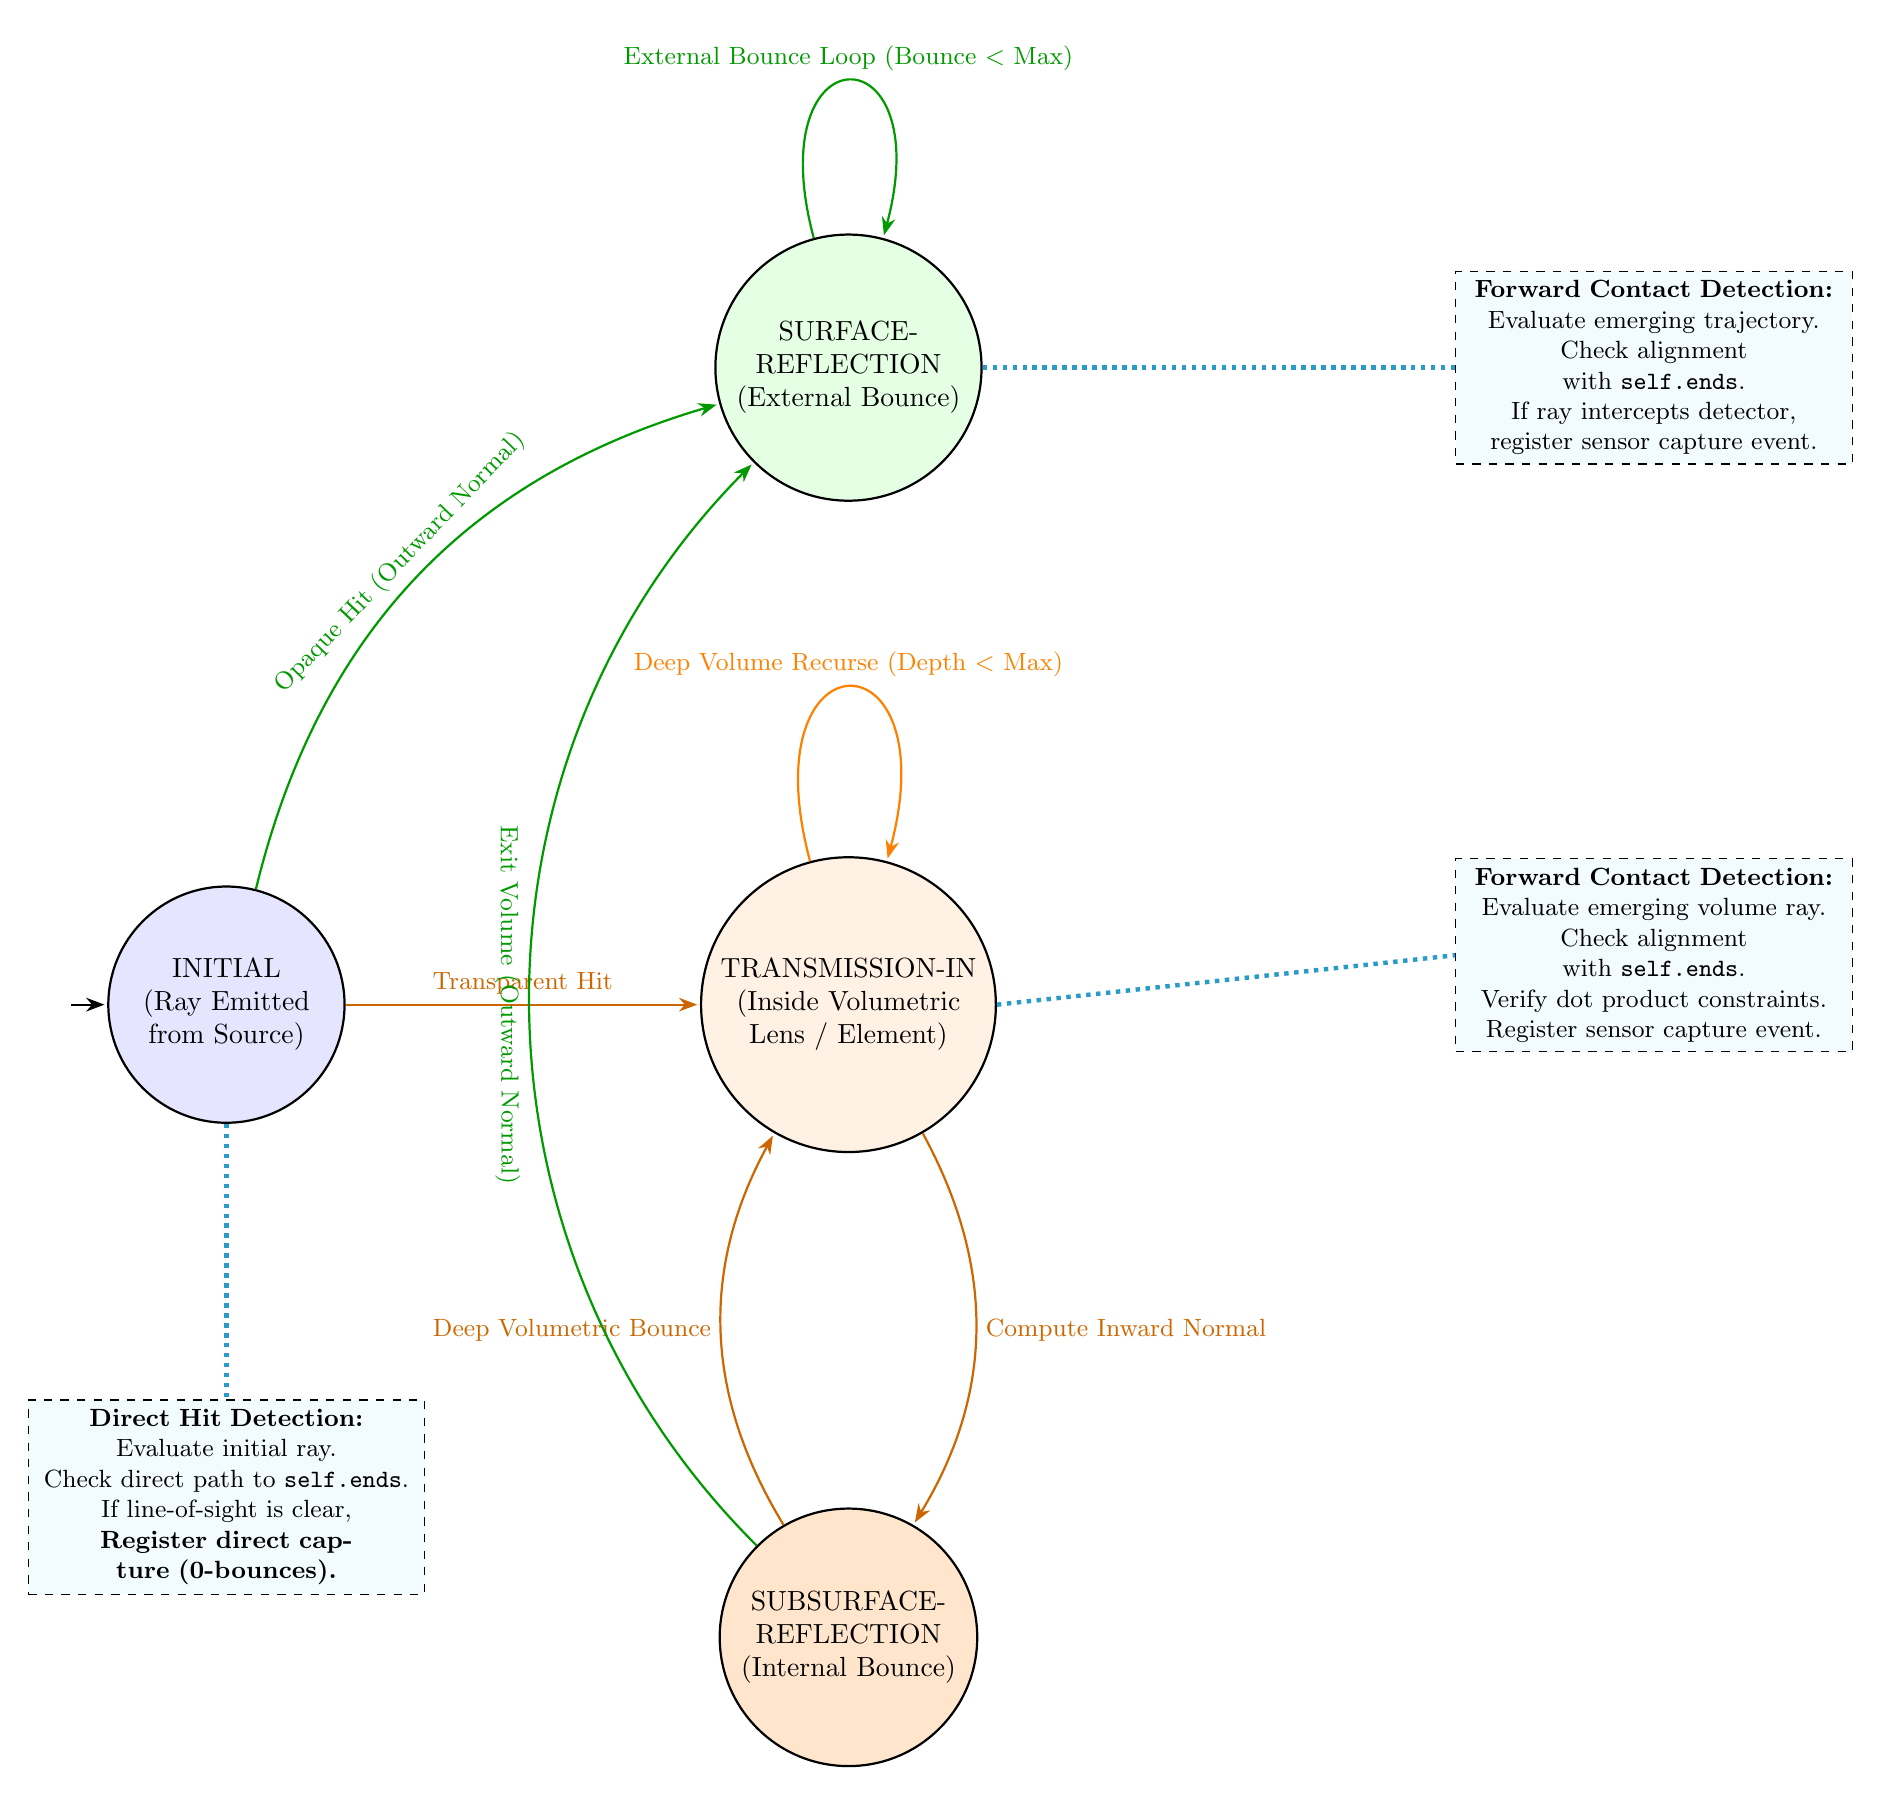
\begin{tikzpicture}[
    >=Stealth,
    node distance=4.5cm,
    every state/.style={thick, fill=blue!10, minimum size=3.0cm, align=center},
    initial text=,
    every edge/.style={draw, ->, thick, shorten >=1pt}
]

    % --- TOPOLOGICAL NODES (Identical Style Grid) ---
    \node[state, initial, initial where=left] (init) {INITIAL\\(Ray Emitted\\from Source)};
    
    % Volumetric (Transmission) States
    \node[state, right=of init, fill=orange!10] (trans_in) {TRANSMISSION-IN\\(Inside Volumetric\\Lens / Element)};
    \node[state, below=of trans_in, fill=orange!20] (sub_ref) {SUBSURFACE-\\REFLECTION\\(Internal Bounce)};
    
    % Surface (Reflection) States
    \node[state, above=of trans_in, fill=green!10] (surf_ref) {SURFACE-\\REFLECTION\\(External Bounce)};

    % --- FORWARD TRACE CONTACT DETECTION OVERLAYS ---
    \node[draw, dashed, fill=cyan!5, text width=4.8cm, align=center, font=\small, below=of init, yshift=1cm] (direct_detect) 
        {\textbf{Direct Hit Detection:}\\Evaluate initial ray.\\Check direct path to \texttt{self.ends}.\\If line-of-sight is clear,\\\textbf{Register direct capture (0-bounces).}};

    \node[draw, dashed, fill=cyan!5, text width=4.8cm, align=center, font=\small, right=of surf_ref, xshift=1.5cm] (surf_detect) 
        {\textbf{Forward Contact Detection:}\\Evaluate emerging trajectory.\\Check alignment with \texttt{self.ends}.\\If ray intercepts detector,\\register sensor capture event.};
        
    \node[draw, dashed, fill=cyan!5, text width=4.8cm, align=center, font=\small, below=of surf_detect, yshift=-0.5cm] (trans_detect) 
        {\textbf{Forward Contact Detection:}\\Evaluate emerging volume ray.\\Check alignment with \texttt{self.ends}.\\Verify dot product constraints.\\Register sensor capture event.};

    % Visual anchors
    \draw[dotted, cyan!80!black, ultra thick] (init.south) -- (direct_detect.north);
    \draw[dotted, cyan!80!black, ultra thick] (surf_ref.east) -- (surf_detect.west);
    \draw[dotted, cyan!80!black, ultra thick] (trans_in.east) -- (trans_detect.west);

    % --- TRANSITIONS & LOGIC FLOW ---
    \path[->] 
        (init) edge[bend left, green!60!black] node[above, sloped, font=\small] {Opaque Hit (Outward Normal)} (surf_ref)
        (init) edge[orange!80!black] node[above, font=\small] {Transparent Hit} (trans_in);

    % Volumetric Loops & Exits
    \path[->]
        (trans_in) edge[loop above, orange] node[above, font=\small] {Deep Volume Recurse (Depth $<$ Max)} (trans_in)
        (trans_in) edge[bend left, orange!80!black] node[right, font=\small] {Compute Inward Normal} (sub_ref)
        (sub_ref) edge[bend left, orange!80!black] node[left, font=\small] {Deep Volumetric Bounce} (trans_in)
        (sub_ref) edge[bend left=45, green!60!black] node[below, sloped, font=\small] {Exit Volume (Outward Normal)} (surf_ref);

    % Surface Loops
    \path[->]
        (surf_ref) edge[loop above, green!60!black] node[above, font=\small] {External Bounce Loop (Bounce $<$ Max)} (surf_ref);

\end{tikzpicture}
\end{document}
